\chapter{Discussion}\label{chp:discussion}

We have now defined the formal structure of the context graph model and have described an algorithm to induce the structure from a given dataset of raw strings. We are now going to discuss some basic principles of how to use the structure as a language model and explore some possible improvements for future applications.
%
\section{Predicting Context by Reconstruction}
%
\begin{figure}[ht!]
\centering
\hspace{-1cm}
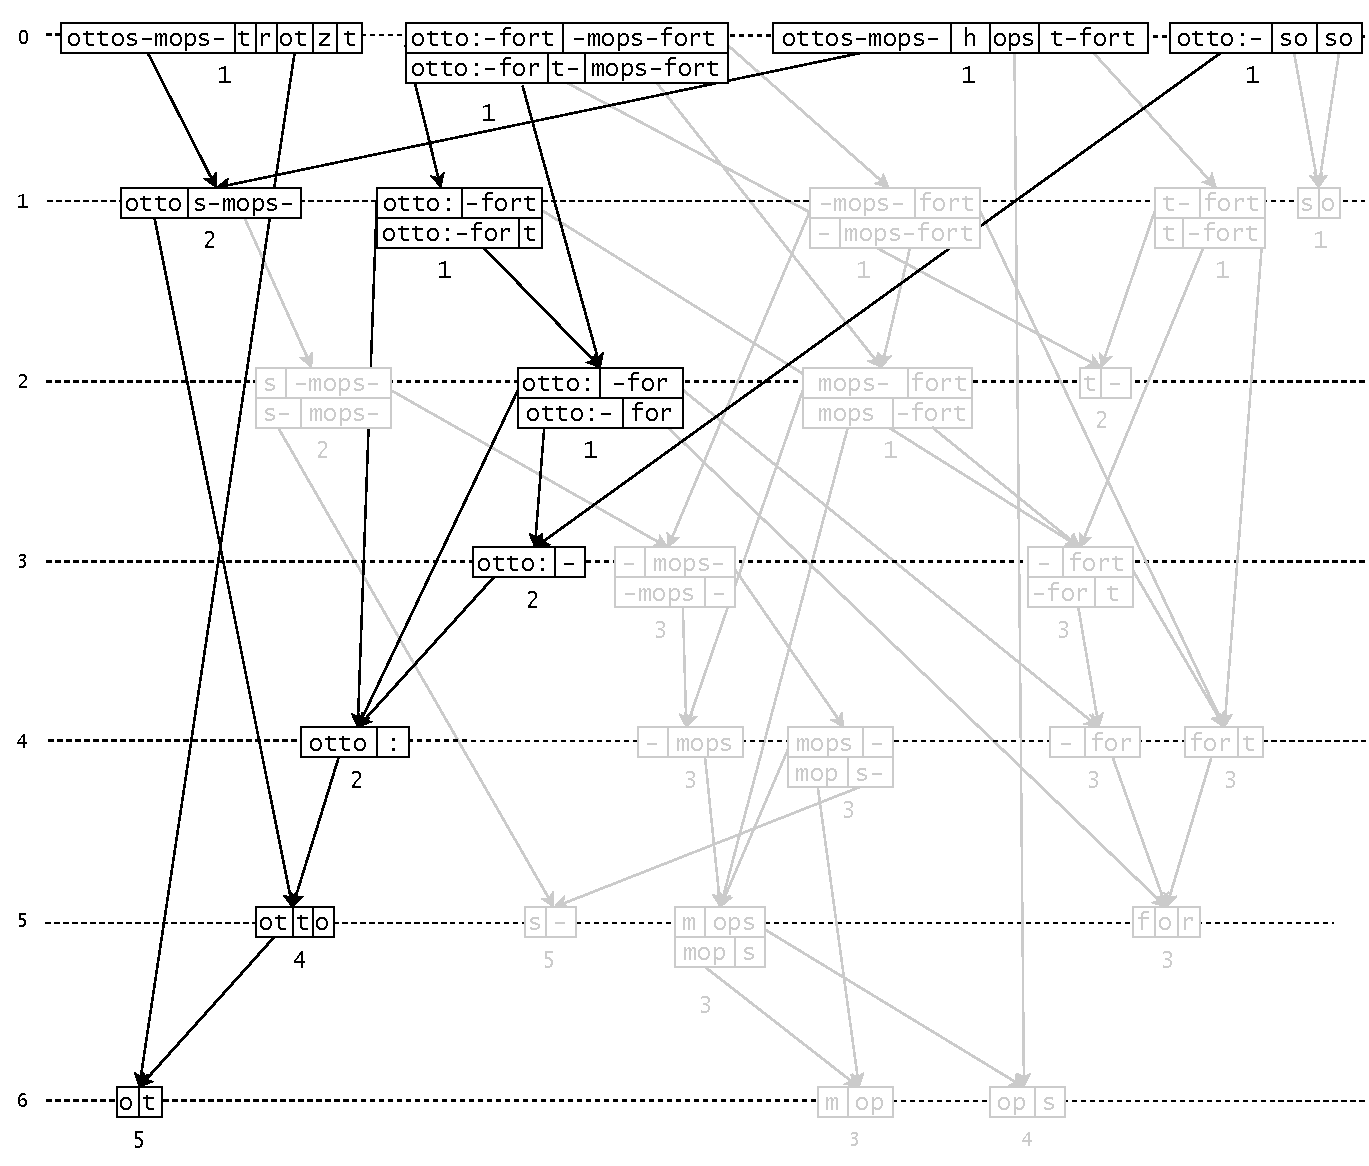
\includegraphics[scale=0.68]{images/ot_subgraph.pdf}
\caption{All available contexts reachable from the node \texttt{ot}.}
\end{figure}
%
\noindent
From the sub-string relation graph we have described, it is easy to model the most likely contexts for a given node in the graph. The conditional probability can be defined identically to regular n-grams.
The probability of a single node can be calculated from the sum of all counts of nodes of the same length $n$, denoted by the set $V_n$:
\begin{align*}
    P(x \mid v) = \dfrac{\texttt{count}(x)}{\texttt{count}(v)} &&
    P(x) = \dfrac{\texttt{count}(x)}{\sum\limits_{v \in V_n}\texttt{count}(v)}
\end{align*}
where $x, v \in V$ are nodes representing strings and $v$ is a sub-string of $x$ in $G$.\par

\noindent
Since the formula for n-gram probabilities in definition~\ref{def:n-gram} can be applied to arbitrary contexts, the same applies to our model. That relationship holds true not only for direct sub-strings in $G$, but any pair of sub- and super-strings. Since all the nodes can generally be viewed as n-grams, the prediction of text can generally work the same as in simple n-gram models, although additional extensions are possible.\\
The key distinction of this structure to n-gram models is that it contains n-grams of all possible lengths from the corpus, while representing them as compressed grammatical rules. The model therefore has a dynamic context window as opposed to classic n-grams which only count a fixed set of n-gram sizes.

\noindent
Additionally, the edges of the graph make it possible to reconstruct the entire original dataset.

\noindent
This way the structure can be used as a basic language model. Given an input over the known alphabet of tokens, there exists a node representing at least the first token, and we can reach its various contexts from this node. With each context annotated with a frequency, we can reconstruct the most frequent context that the given prefix is known to occur in.

\noindent
In the following example the node $\texttt{ot}$ has different contexts each of a different frequency. It occurs directly in \texttt{ottos-mops-tr\underline{ot}zt} and in \texttt{\underline{ot}to}. For predicting the most likely completion an algorithm could pick the most frequent of the available contexts to predict the next tokens, the same way as an n-gram model.

\begin{multicols}{2}
    \noindent
    \begin{align*}
        P\left(\texttt{to} \mid \texttt{ot}\right) = \frac{4}{5}
    \end{align*}
    \begin{align*}
        P\left(\texttt{zt} \mid \texttt{ot}\right) = \frac{1}{5}
    \end{align*}
\end{multicols}
%
\noindent
Compared to alternative language modelling approaches, our structure has these specific advantages due to its explicit symbolic structure, efficient representation and dynamic construction procedure, illustrated by the following table:

\begin{table}[!h]
\centering
    \begin{tblr}{
        colspec=l|c|c|c,
        hline{2}=solid,
    }
        &N-Grams&Transformers&Context Graph\\
        reconstructable&\xmark&\xmark&\cmark\\
        interpretable&\cmark&\xmark&\cmark\\
        updatable&\cmark&\xmark&\cmark\\
        dynamic context size&\xmark&\xmark&\cmark
    \end{tblr}
\caption{Comparison chart of different language modelling techniques regarding properties discussed in the paper.}
\end{table}

\section{Smoothing Techniques}
As with regular n-grams, especially for larger n-grams, data sparsity can be a problem for sensible predictions. As the size of the context grows, the possibilities for different sequences rises exponentially and a training data set will simply not cover all variations of valid phrases. This can also be considered an advantage as it keeps the model within the predefined boundaries it was trained on, however for most applications we want the model to be robust to unseen inputs and be able to handle them appropriately.

One way to allow for responses to unseen inputs of the model is to \textit{smooth} the probability distribution by exploring \textit{similar} n-grams when sampling from the model by some similarity measure. Naive smoothing approaches simply assign all possible n-grams an artificial minimal count to prevent any probabilities to be zero and allow for n-grams which have never been seen in practice to be generated (Laplace Smoothing). These techniques however do not utilize the syntactic or semantic similarity of the n-grams, as would be intuitive, and thus create noise in the output.
In practice, we assume the training data to be a subset of a language following some hidden rules and being modified by random noise (such as spelling errors). Thus, we would assume a higher probability for n-grams which are similar to the instances we have actually seen during training.

\subsection{Syntactic Similarity}
Similarity of texts can be defined in terms of syntactic structure or in terms of semantic meaning, which by the distributional hypothesis refers to the similarity of the contexts they occur in.

\noindent
The syntactic similarity of two texts is usually quantified by their distance in a space over edit operations, also called edit distance. There are several types of edit distance, depending on which edit operations are allowed and how they are counted. We are going to assume the \textit{Levenshtein Distance} for this example.

\dfn{Levenshtein Distance}{
    The Levenshtein Distance $\text{lev}(x_1, x_2)$ of two texts $x_1$, $x_2$ is the minimum number of \textbf{insertions}, \textbf{deletions} or \textbf{substitutions} of characters needed to transform one text into the other.
    
    A syntactic similarity metric can then be defined as
    
    \begin{align*}
        \text{sim}_\text{orth}(x_1, x_2) = 1 - \frac{\text{lev}(x_1, x_2)}{\max\{|x_1|, |x_2|\}}
    \end{align*}
    where $\max\{|x_1|, |x_2|\}$ gives the maximum possible Levenshtein distance for $x_1$ and $x_2$. Thus, the similarity ranges between 0 and 1.
}
\noindent
A core advantage of the substring structure is the ability to easily traverse the most similar nodes according to the Levenshtein distance. We can derive an upper bound for the distance (or lower bound of syntactic similarity) for the most similar n-grams utilizing the sub-string relation.

\dfn{Edit-Distance in $G$}{
    For the edit distance $\text{lev}(x_1, x_2): V \times V \rightarrow \NN$ of two nodes $x_1, x_2 \in V$ is
    \begin{itemize}
        \item $\text{lev}(x_1, x_2) = ||x_1| - |x_2||$ if one is a sub-string of the other,
        \item $\text{lev}(x_1, x_2) \leq \text{lev}(x_1, x_3) + \text{lev}(x_2, x_3)$ if there exists a shared sub-string $x_3$ 
        \item $\text{lev}(x_1, x_2) = \max\{|x_1|, |x_2|\}$ if there are no shared sub-strings
    \end{itemize}
}
\noindent
Because each node is connected to its largest sub-strings and smallest super-strings, we can traverse the set of syntactically similar strings in a similarity-descending order by visiting the super-strings of sub-strings. With each edge traversed we either add to or remove a minimal amount of context from a given node and explore neighborhoods of the largest shared substrings first.

\subsection{Semantic Similarity}
The semantic similarity of two texts can be defined on lexical terms as the similarity of the possible contexts the texts may appear in. Thus, the semantic distance of two distinct n-grams can be defined as the average syntactic edit-distance between all of their contexts:
\dfn{Semantic Distance}{
    The semantic distance $\text{dist}_\text{sem}(x_1, x_2): V \times V \rightarrow \NN$ of two nodes $x_1, x_2 \in V$ is the average minimum edit distance between contexts of $x_1$ and $x_2$
    \begin{align*}
        \text{dist}_\text{sem}(x_1, x_2) \coloneqq \text{avg}(\{\min\{\text{lev}(c_1, c_2) \mid c_2 \in \text{Ctx}(x_2)\} \mid c_1 \in \text{Ctx}(x_1)\})
    \end{align*}
}
\noindent
The semantic distance captures the syntactic edit operations required to
transform the known contexts of one text into the contexts of the other text and
thus quantifies their degree of compatibility with the remaining corpus.

\noindent
Similarly to how attention weights in a self-attention unit of the transformer architecture are trained to point to their contexts in a hyper-dimensional latent space, the nodes in a sub-string relation are linked with other strings they appear in context with. By comparing the similarity of these links we can quantify the semantic similarity by the same definition of distributional semantics.

\noindent
One difference is that in the self-attention mechanism, tokens link to other tokens, even when they never appear in the same context during training. When $a$ and $b$ appear in the same context and thus $a$ is weighed towards $b$, $a$ is also weighed towards tokens similar to $b$ even if they have never been seen in the same contexts.

\noindent
To replicate this behaviour in the sub-string relation graph, we can modify the edit distance of contexts to discount replacements with high semantic similarity. The semantic distance between two texts should be lower when the contexts can be transformed into one another using semantically similar nodes.

\noindent
To find the semantically most similar nodes to a given node, we find the possible replacements for it in its contexts. This can be achieved by finding the alternative contexts for each context node of the original node. In a recursive procedure we keep traversing the sub-string relation in a breadth-first manner until we find nodes with no contexts or no children, keeping track of the minimum path lengths for each transformation. Because the structure stores direct edges between the most similar sub-strings, paths between most similar nodes will be shortest and a lower bound for similarity can be placed on transformations not fully explored. This way the semantic similarity of nodes can be incrementally approximated according to resource requirements.

\section{Accepting Novel Inputs}
For inputs seen in the training corpus it is easy to predict the appropriate context, as there exists a node in the graph structure to derive contexts from. However, in general, input strings can be composed of novel combinations of tokens which have only partially been seen in training, if at all. To allow the model to predict context for unknown sequences, we need to allow it to draw information from nodes similar to the input.

A simple way to address this in common n-gram models is to use \textit{backoff smoothing}. 

\dfn{Backoff Smoothing}{
    The Backoff probability of an n-gram $w_{i - n + 1}, \ldots, w_i$ is defined as
    \begin{align*}
        P_{bo}(w_i \mid w_{i - n + 1}, \ldots, w_{i-1})
        =\begin{dcases}
            \frac{C(w_{i - n + 1}, \ldots, w_i)}{C(w_{i - n + 1}, \ldots, w_{i-1})} &\text{ if } C(w_{i - n + 1}, \ldots, w_i) > 0,\\
            P_{bo}(w_i \mid w_{i - n + 2}, \ldots, w_{i-1}) &\text{ otherwise}
        \end{dcases}
    \end{align*}
    Meaning the length of context to be conditioned upon will be reduced as long
    as there exists no support for the resulting n-gram in the model. Instead, the n-gram probability of the largest context available in the model is used.
}
We could apply the same form of smoothing in the hierarchy of the sub-string relation, but it would certainly be better to search for nodes syntactically or semantically similar to the input and use their contexts for prediction instead.